\documentclass[10pt]{article}
\usepackage{blindtext}
\usepackage{graphicx}
\usepackage{array}
\setlength{\parindent}{0em}
\newcolumntype{P}[1]{>{\centering\arraybackslash}p{#1}}
\graphicspath{ {/Users/Xiaopei/Documents/Coursework/Fall\ 2017/STATS\ M231/Project\ 0/Report}}
\usepackage[margin=1in]{geometry}
\title{Project 0: Classification by Deep Learning}
\author{Xiaopei Zhang (004309991)}
\date{\today}
\begin{document}
\maketitle
\section*{\small{Task 1: Train full LeNet, plot training/testing error}}
	Download the CIFAR-10 Dataset, and train a LeNet on it. Plot the training error and the validation error against the training epoch (Figure 1). \\
	\begin{figure}[h]
		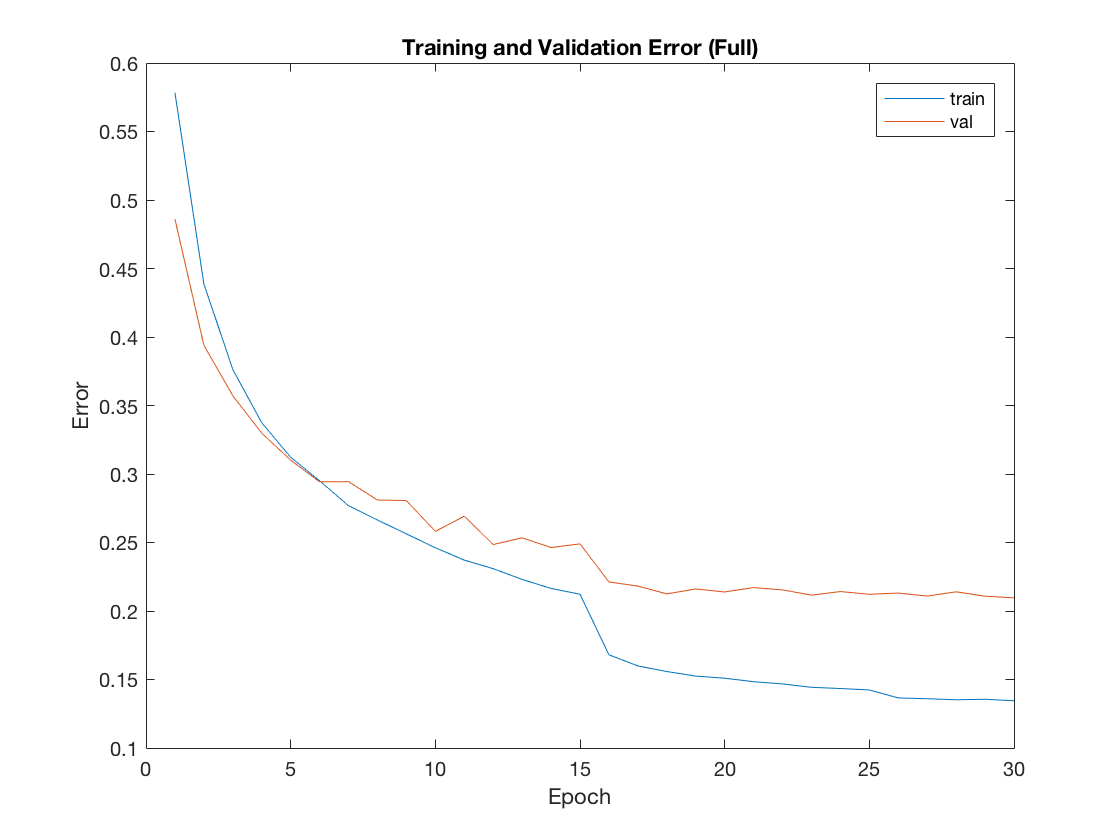
\includegraphics[width=\textwidth]{full_error}
		\caption{Training and validation errors for full training.}
		\label{1}
	\end{figure}
\section*{\small{Task 2: Remove blocks}}
	Keep Block5, and train a modified LeNet with only: i) Block1; ii) Block1 and Block2; iii) Block1, Block2 and Block3 respectively. Record the final training and validation errors (Table 1). \\
	\begin{table}
 		\centering
 		\begin{tabular}{|c|c|c|c|c|}
		\hline
		LeNet Structure & Full & i) & ii) & iii) \\ \hline
		Training Error & 0.1344800 & 0.7318000 & 0.4462000 & 0.3275800  \\ \hline
		Validation Error & 0.2096000 & 0.7353200 & 0.4583000 & 0.3282000 \\ \hline
 		\end{tabular}
		\caption{Training and validation errors for different LeNet structures.}\label{tab1}
	\end{table}\\
	From Table 1, we observe that as the number of hidden layers (blocks) of LeNet increases, both training and validation errors decrease.
\section*{\small{Task 3: Visualize filter response}}
For each image, visualize the filter response maps of 32 filters in the first layer of LeNet. \\
Image 1:
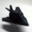
\includegraphics{1}\\
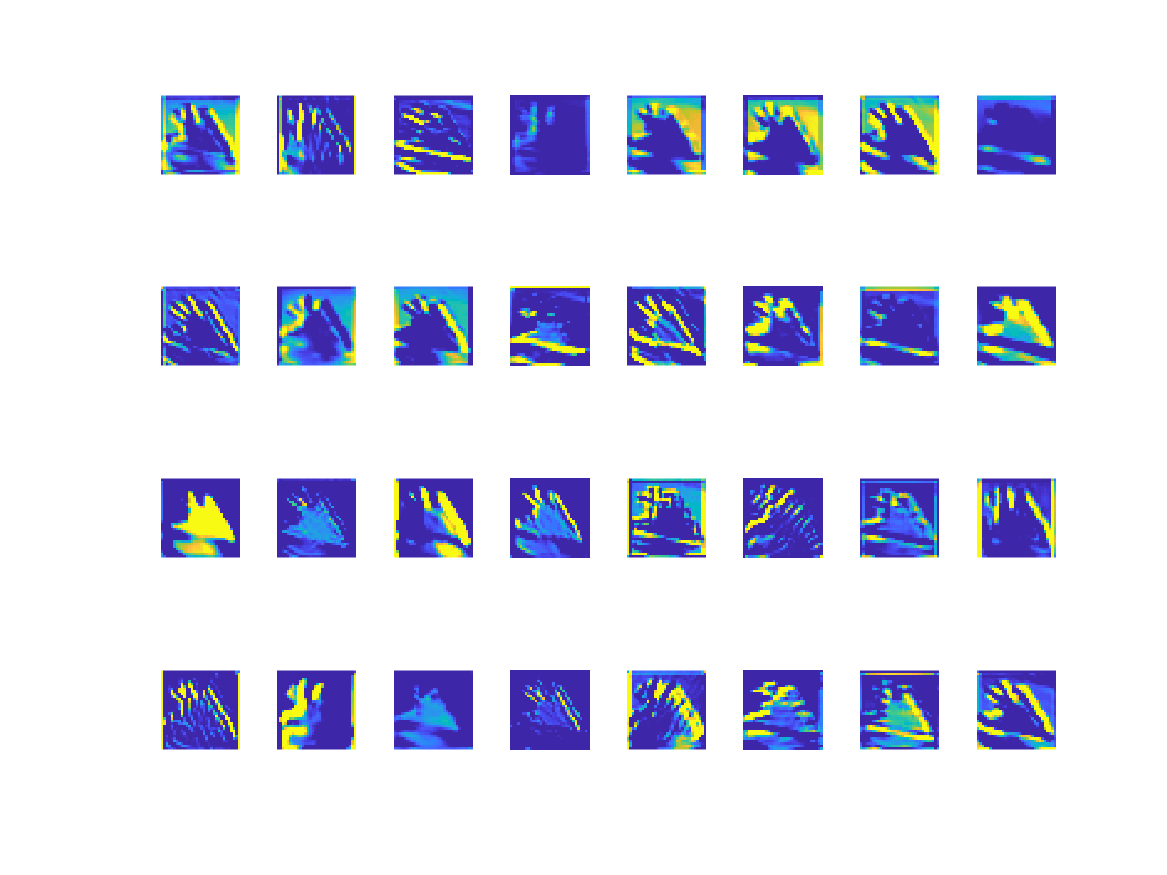
\includegraphics[scale=0.65]{1_filter_res}\\
\newpage
Image 2:
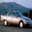
\includegraphics{2}\\
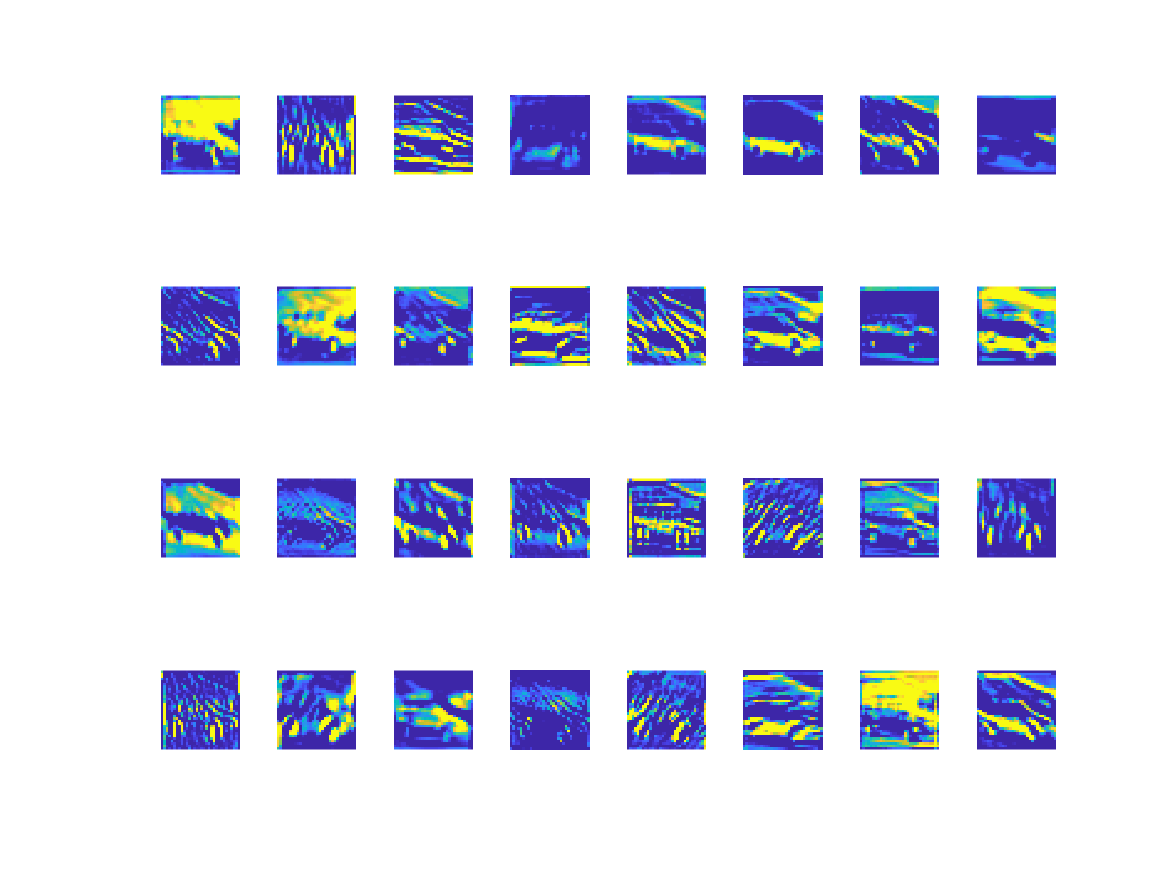
\includegraphics[scale=0.65]{2_filter_res}\\
Image 3:
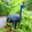
\includegraphics{3}\\
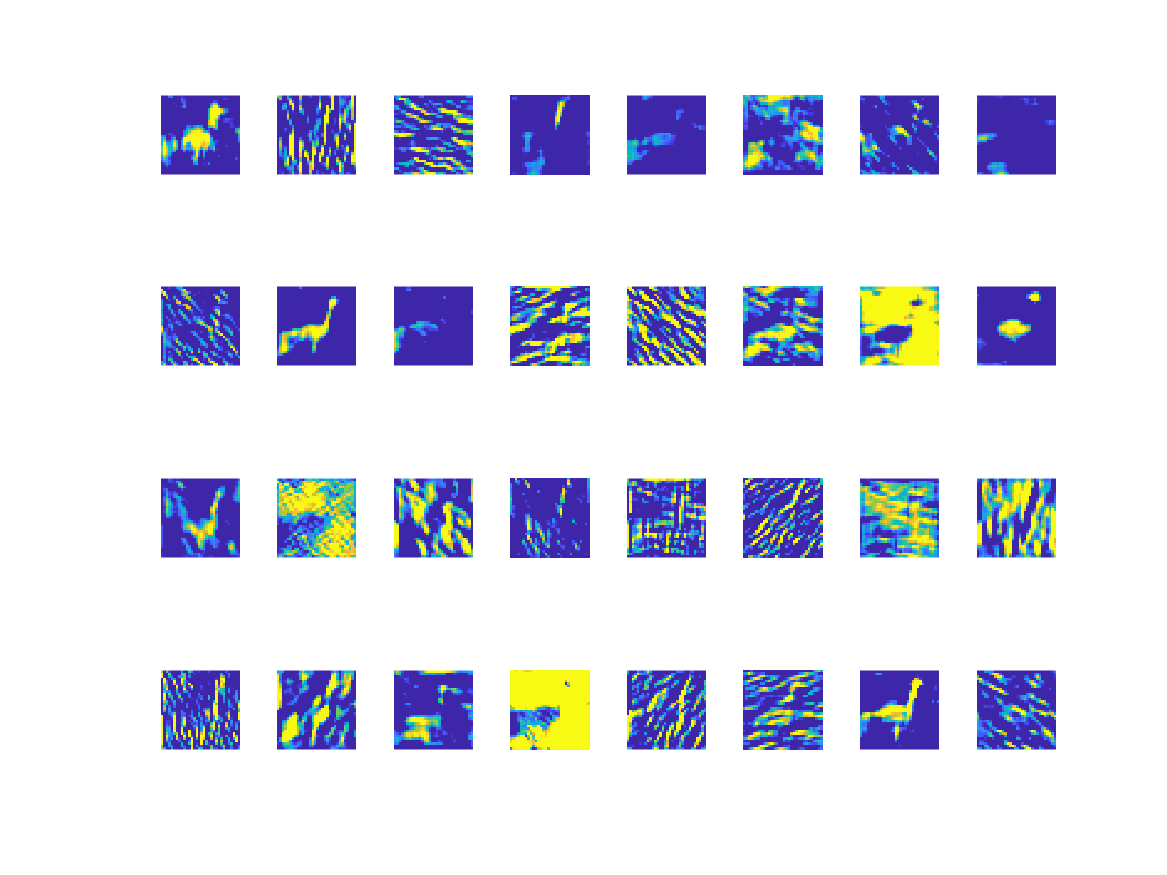
\includegraphics[scale=0.65]{3_filter_res}\\
\newpage
Image 4:
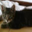
\includegraphics{4}\\
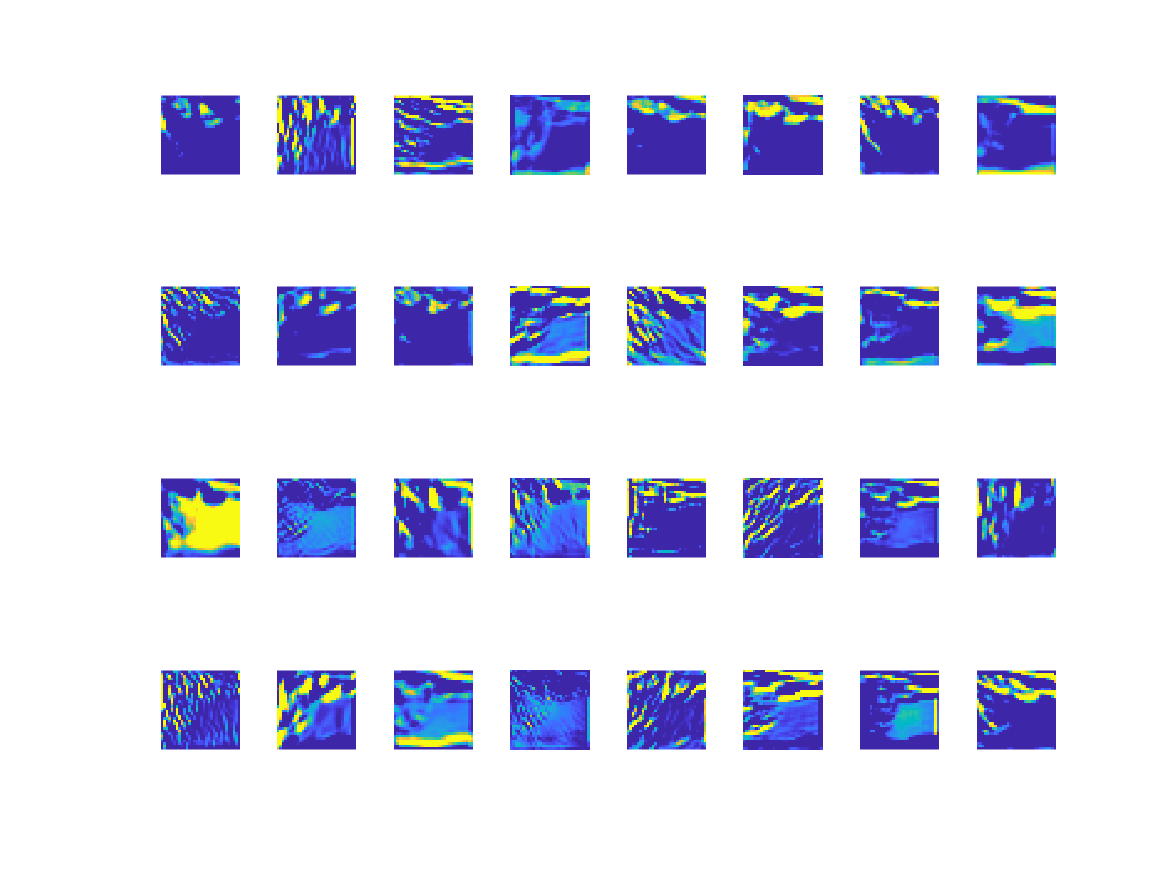
\includegraphics[scale=0.65]{4_filter_res}\\
Image 5:
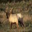
\includegraphics{5}\\
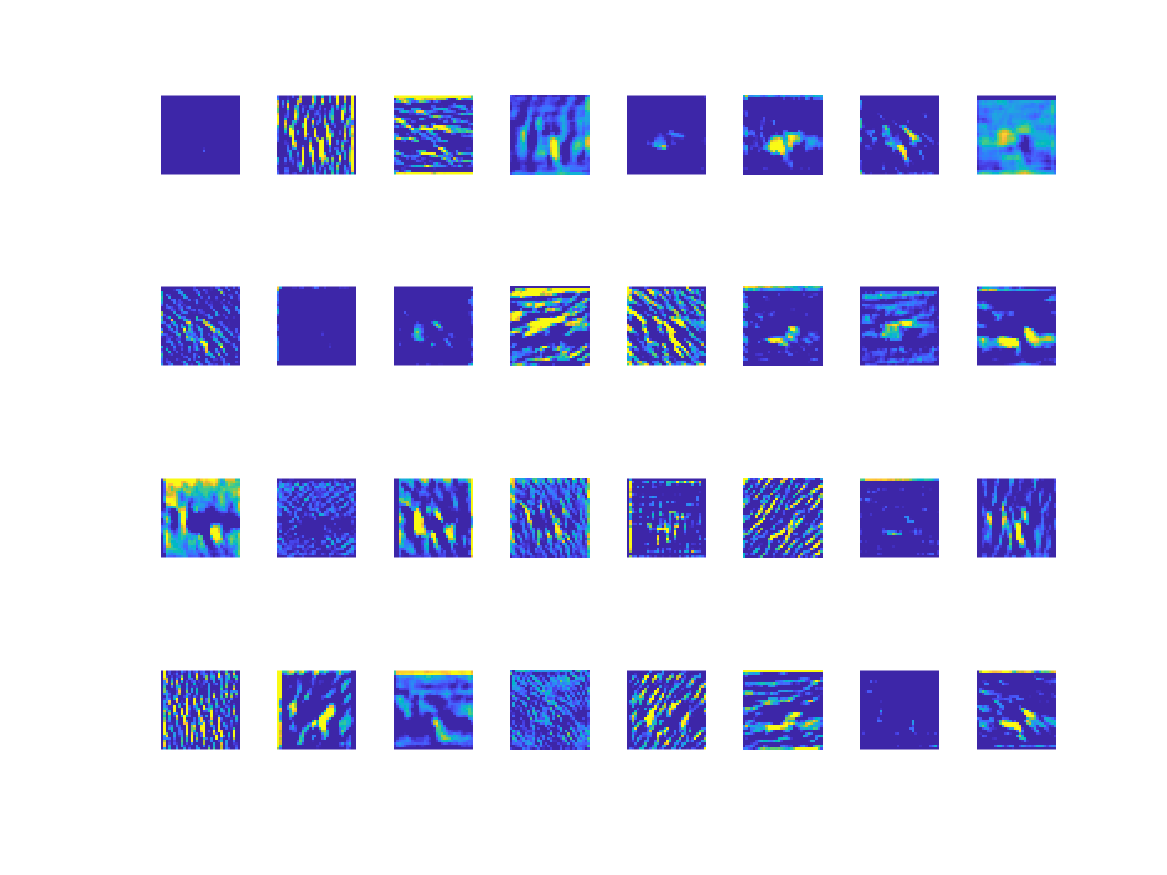
\includegraphics[scale=0.65]{5_filter_res}\\
\newpage
Image 6:

\includegraphics{6}\\
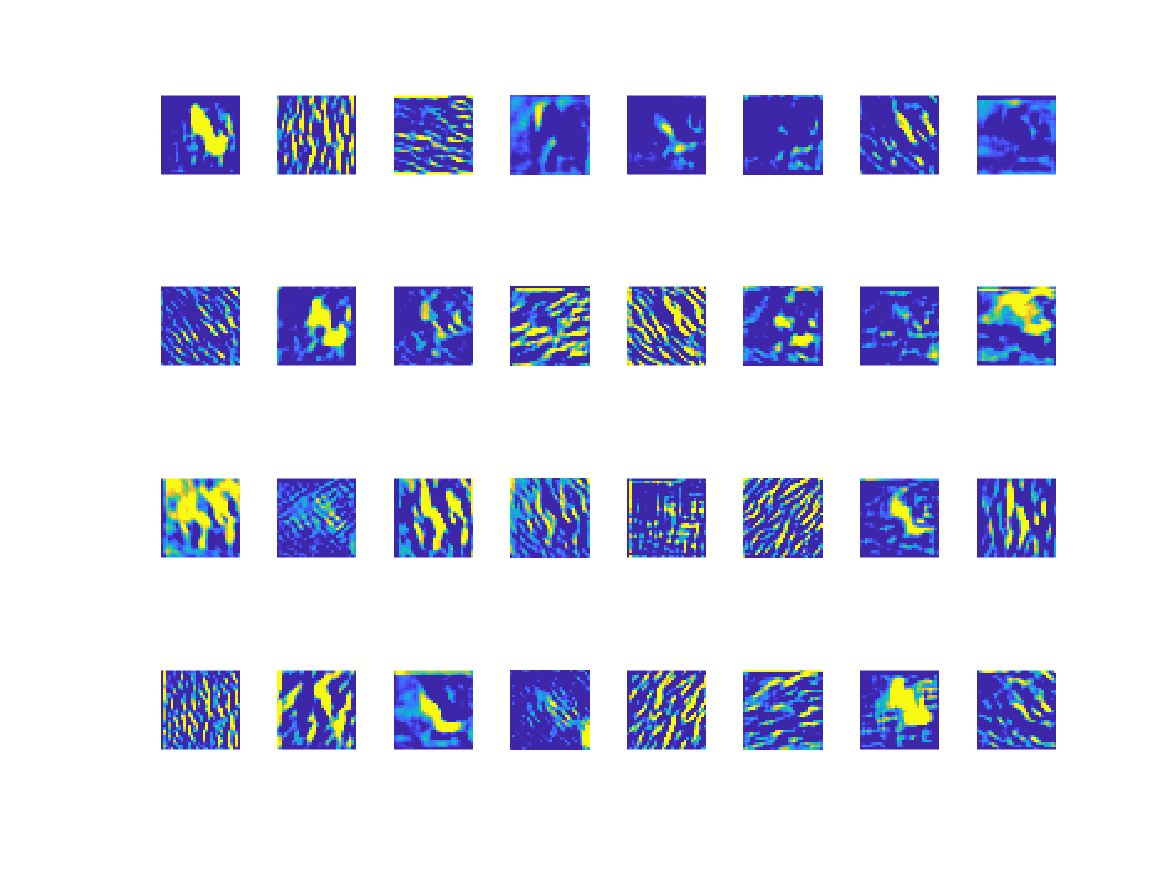
\includegraphics[scale=0.65]{6_filter_res}\\
Image 7:

\includegraphics{7}\\
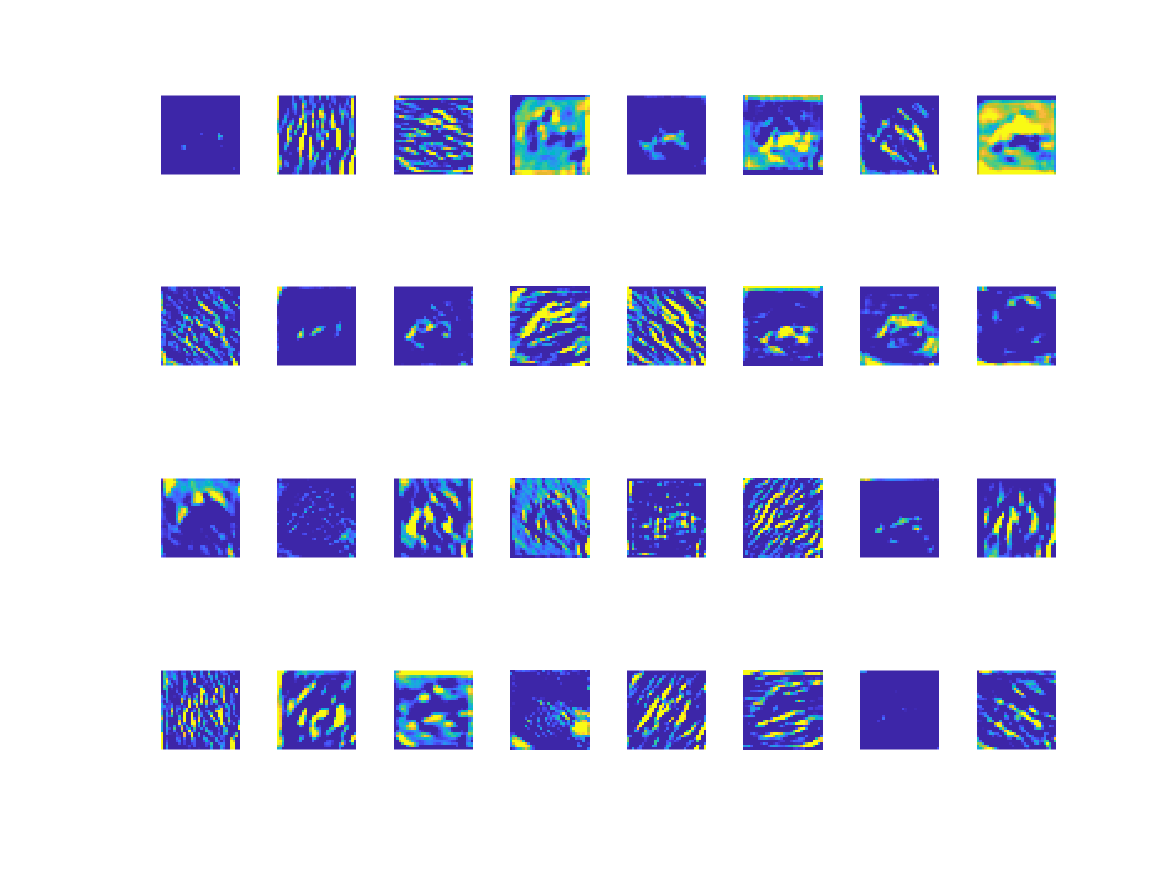
\includegraphics[scale=0.65]{7_filter_res}\\
\newpage
Image 8:

\includegraphics{8}\\
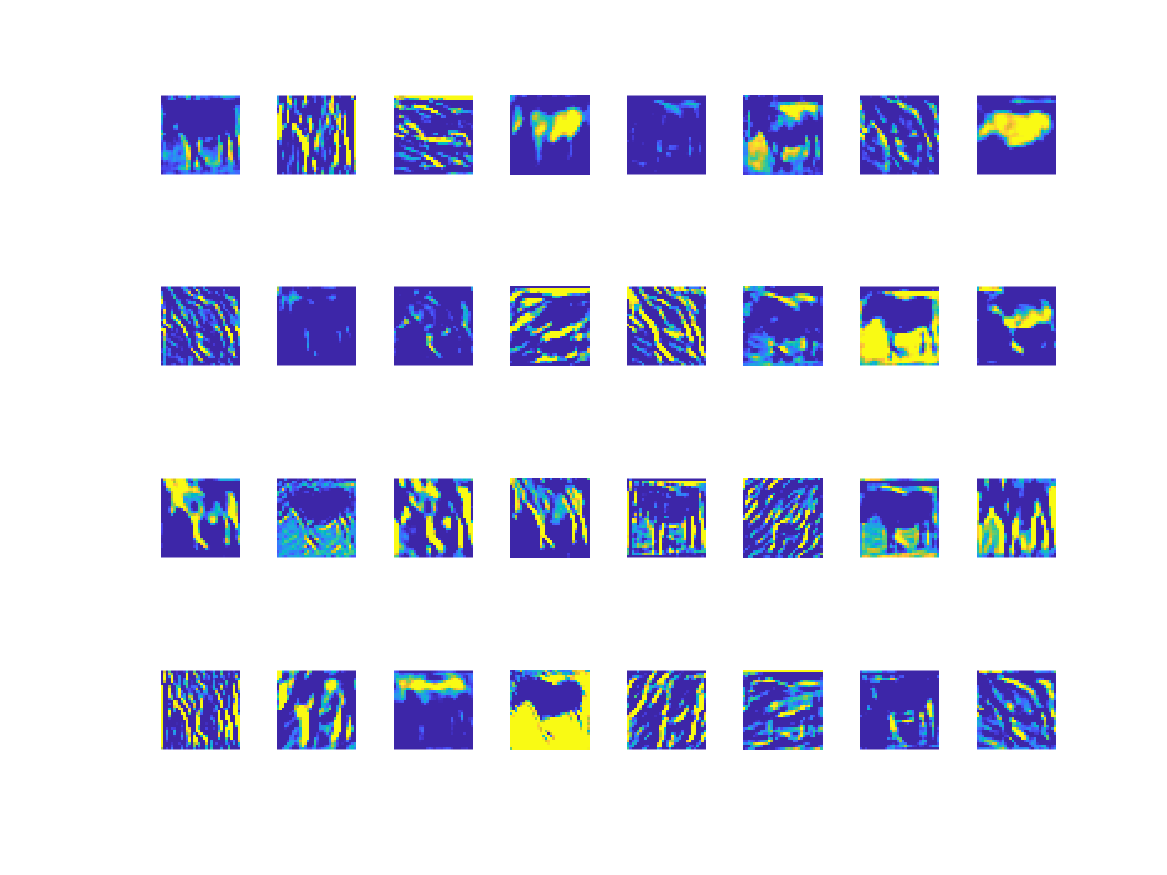
\includegraphics[scale=0.65]{8_filter_res}\\
Image 9:

\includegraphics{9}\\
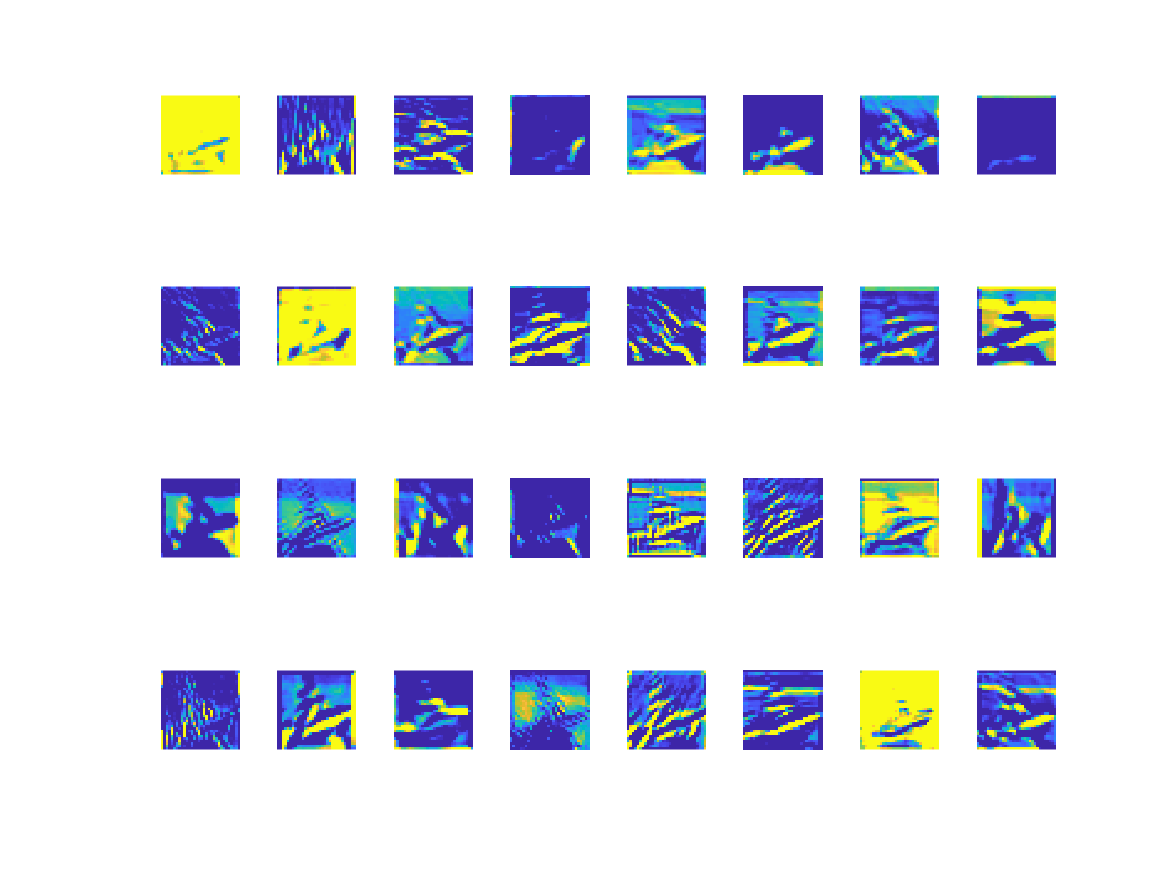
\includegraphics[scale=0.65]{9_filter_res}\\
\newpage
Image 10:
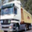
\includegraphics{10}\\
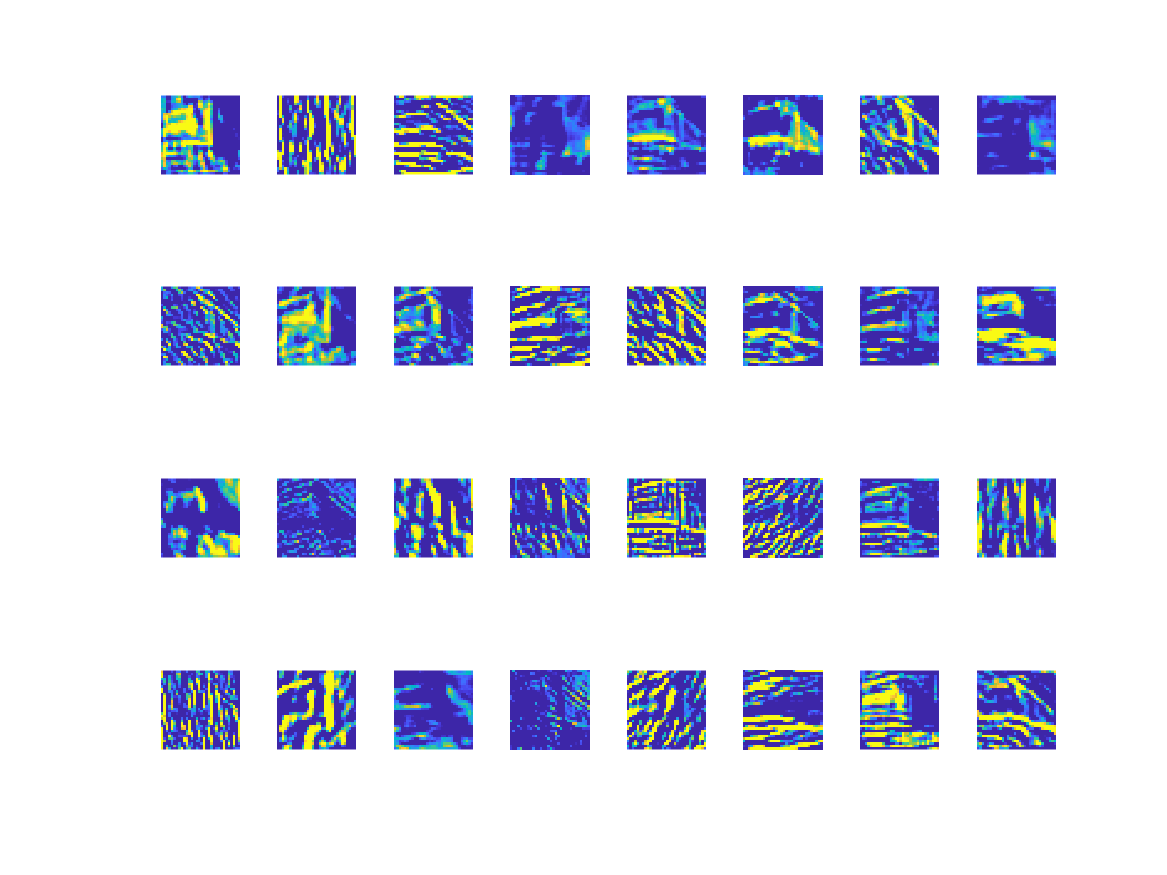
\includegraphics[scale=0.65]{10_filter_res}\\
\end{document}